%% if you are submitting an initial manuscript then you should have submission as an option here
%% if you are submitting a revised manuscript then you should have revision as an option here
%% otherwise options taken by the article class will be accepted
\documentclass[submission]{FPSAC2025}
%% but DO NOT pass any options (or change anything else anywhere) which alters page size / layout / font size etc

%% note that the class file already loads {amsmath, amsthm, amssymb}

\usepackage{xargs}
\usepackage{hypcap}
\usepackage{paralist}
\usepackage{dsfont}
\usepackage{mathtools}
\usepackage{blkarray}
\usepackage{picins/picins}
\usepackage{overpic}

% theorems
\newtheorem{theorem}{Theorem}%[section]
\newtheorem{corollary}[theorem]{Corollary}
\newtheorem{proposition}[theorem]{Proposition}
\newtheorem{lemma}[theorem]{Lemma}
\newtheorem{conjecture}[theorem]{Conjecture}
\newtheorem*{theorem*}{Theorem}%[section]
\newtheorem*{proposition*}{Proposition}%[section]
\newtheorem*{conjecture*}{Conjecture}%[section]

\theoremstyle{definition}
\newtheorem{definition}[theorem]{Definition}
\newtheorem{example}[theorem]{Example}
\newtheorem{remark}[theorem]{Remark}
\newtheorem{question}[theorem]{Question}
\newtheorem{problem}[theorem]{Problem}
\newtheorem{notation}[theorem]{Notation}
\newtheorem{assumption}[theorem]{Assumption}
\newtheorem{defprop}[theorem]{Definition/Proposition}
\newtheorem{warning}[theorem]{Warning}
\crefname{notation}{Notation}{Notations}
\crefname{problem}{Problem}{Problems}
 
% math special letters
\newcommand{\R}{\mathbb{R}} % reals
\newcommand{\N}{\mathbb{N}} % naturals
\newcommand{\Z}{\mathbb{Z}} % integers
\newcommand{\C}{\mathbb{C}} % complex
\newcommand{\I}{\mathbb{I}} % set of integers
\newcommand{\HH}{\mathbb{H}} % hyperplane
\newcommand{\K}{\mathbb{K}} % field
\newcommand{\fA}{\mathfrak{A}} % alternating group
\newcommand{\fB}{\mathfrak{S}^\textsc{b}} % signed symmetric group
\newcommand{\cA}{\mathcal{A}} % algebra
\newcommand{\cC}{\mathcal{C}} % collection
\newcommand{\cS}{\mathcal{S}} % ground set
\newcommand{\uR}{\underline{R}} % underline set
\newcommand{\uS}{\underline{S}} % underline set
\newcommand{\uT}{\underline{T}} % underline set
\newcommand{\oS}{\overline{S}} % overline set
\newcommand{\ucS}{\underline{\cS}} % underline ground set
\renewcommand{\c}[1]{\mathcal{#1}} % caligraphic letters
\renewcommand{\b}[1]{{\boldsymbol{#1}}} % bold letters
\newcommand{\bb}[1]{\mathbb{#1}} % bb letters
\newcommand{\f}[1]{\mathfrak{#1}} % frak letters
\newcommand{\h}{\widehat} % hat letters

% math commands
\newcommand{\set}[2]{\left\{ #1 \;\middle|\; #2 \right\}} % set notation
\newcommand{\bigset}[2]{\big\{ #1 \;\big|\; #2 \big\}} % big set notation
\newcommand{\Bigset}[2]{\Big\{ #1 \;\Big|\; #2 \Big\}} % Big set notation
\newcommand{\setangle}[2]{\left\langle #1 \;\middle|\; #2 \right\rangle} % set notation
\newcommand{\ssm}{\smallsetminus} % small set minus
\newcommand{\dotprod}[2]{\left\langle \, #1 \; \middle| \; #2 \, \right\rangle} % dot product
\newcommand{\symdif}{\,\triangle\,} % symmetric difference
\newcommand{\one}{\b{1}} % the all one vector
\newcommand{\eqdef}{\mbox{\,\raisebox{0.2ex}{\scriptsize\ensuremath{\mathrm:}}\ensuremath{=}\,}} % :=
\newcommand{\defeq}{\mbox{~\ensuremath{=}\raisebox{0.2ex}{\scriptsize\ensuremath{\mathrm:}} }} % =:
\newcommand{\simplex}{\b{\triangle}} % simplex
\renewcommand{\implies}{\Rightarrow} % imply sign
\newcommand{\transpose}[1]{{#1}^t} % transpose matrix

% operators
\DeclareMathOperator{\conv}{conv} % convex hull
\DeclareMathOperator{\vect}{vect} % linear span
\DeclareMathOperator{\cone}{cone} % cone hull
\DeclareMathOperator{\inv}{inv} % inversions
\DeclareMathOperator{\ninv}{ninv} % inversions
\DeclareMathOperator{\Ima}{Im} % image
\DeclareMathOperator{\Vol}{Vol} % (mixed) volume
\DeclareMathOperator{\Hom}{Hom} % hom-spaces
\DeclareMathOperator{\Ext}{Ext} % extensions

% others
\newcommand{\ie}{\textit{i.e.}~} % id est
\newcommand{\eg}{\textit{e.g.}~} % exempli gratia
\newcommand{\Eg}{\textit{E.g.}~} % exempli gratia
\newcommand{\apriori}{\textit{a priori}} % a priori
\newcommand{\viceversa}{\textit{vice versa}} % vice versa
\newcommand{\versus}{\textit{vs.}~} % versus
\newcommand{\aka}{\textit{a.k.a.}~} % also known as
\newcommand{\perse}{\textit{per se}} % per se
\newcommand{\ordinal}{\textsuperscript{th}} % th for ordinals
\newcommand{\ordinalst}{\textsuperscript{st}} % st for ordinals
\definecolor{darkblue}{rgb}{0,0,0.7} % darkblue color
\definecolor{green}{RGB}{57,181,74} % darkblue color
\definecolor{violet}{RGB}{147,39,143} % darkblue color
\newcommand{\darkblue}{\color{darkblue}} % darkblue command
\newcommand{\defn}[1]{\textsl{\darkblue #1}} % emphasis of a definition
\newcommand{\para}[1]{\smallskip\noindent\uline{#1.}} % paragraph
\renewcommand{\topfraction}{1} % possibility to have one page of pictures
\renewcommand{\bottomfraction}{1} % possibility to have one page of pictures
%\renewcommand\labelitemi{$\diamond$} % redefine itemize default symbol

% marginal comments
\usepackage{todonotes}
\newcommand{\vincent}[1]{\todo[color=blue!30]{\rm #1 \\ \hfill --- V.}}
\newcommand{\asilata}[2][]{\todo[size=\scriptsize, color=orange!30,#1]{\rm #2 \\ \hfill --- A.}}

% lattices
\newcommand{\meet}{\wedge} % meet
\newcommand{\join}{\vee} % join
\newcommand{\bigMeet}{\bigwedge} % meet
\newcommand{\bigJoin}{\bigvee} % join
\newcommandx{\projDown}[1][1={}]{\smash{\pi_\downarrow^{#1}}} % down projection map
\newcommandx{\projUp}[1][1={}]{\smash{\pi^\uparrow_{#1}}} % up projection map
\newcommand{\con}{\mathrm{con}} % congruence

% geometry
\newcommandx{\Fan}[1][1=D]{\mathcal{F}_{#1}} % fan
\newcommand{\polytope}[1]{\mathds{#1}} % font polytope

% specific wiggly
\newcommand{\wigglyComplex}{\mathrm{WC}} % wiggly complex
\newcommand{\wigglyFlipGraph}{\mathrm{WFG}} % wiggly flip graph
\newcommand{\wigglyIncreasingFlipGraph}{\mathrm{WIFG}} % wiggly increasing flip graph
\newcommand{\wigglyLattice}{\mathrm{WL}} % wiggly lattice
\newcommand{\wigglyFan}{\mathrm{WF}} % wiggly fan
\newcommand{\wigglyhedron}{\polytope{W}} % wigglyhedron
\newcommand{\Asso}{\polytope{A}\mathsf{sso}} % associahedron

\graphicspath{{figures/}}

%% define your title in the usual way
\title{Wigglyhedra}

%% define your authors in the usual way
%% use \addressmark{1}, \addressmark{2} etc for the institutions, and use \thanks{} for contact details
%% for more than 3 names, use the Oxford comma: One Author, Two Author, Red Author, \and Blue Author
\author{Asilata Bapat\thanks{\href{mailto:asilata.bapat@anu.edu.au}{mailto:asilata.bapat@anu.edu.au}. Supported by the Australian DECRA grant DE240100447.}\addressmark{1} \and Vincent Pilaud\thanks{\href{mailto:vincent.pilaud@ub.edu}{mailto:vincent.pilaud@ub.edu}. Supported by the French--Austrian grant PAGCAP (ANR-21-CE48-0020 \& FWF I 5788) and by the Spanish grant PID2022-137283NB-C21.}\addressmark{2}}

%% then use \addressmark to match authors to institutions here
\address{\addressmark{1}The Australian National University, Canberra, Australia \\ \addressmark{2}Universitat de Barcelona, Spain}

%% put the date of submission here
\received{\today}

%% leave this blank until submitting a revised version
%\revised{}

%% put your English abstract here, or comment this out if you don't have one yet
%% please don't use custom commands in your abstract / resume, as these will be displayed online
%% likewise for citations -- please don't use \cite, and instead write out your citation as something like (author year)
\abstract{Motivated by categorical representation theory, we study the wigglyhedron. Its boundary complex encodes wiggly dissections (sets of pairwise pointed and non-crossing arcs wiggling around $n+2$ points on a line). Its graph is the Hasse diagram of the sublattice of the weak order induced by wiggly permutations (permutations of $[2n]$ avoiding~$2j-1 \cdots i \cdots 2j$ for~$i < 2j-1$ and~$2j \cdots k \cdots 2j-1$ for~$k > 2j$). It contains copies of all type~$A_n$ Cambrian lattices and Cambrian fans.}

%% put your French abstract here, or comment this out if you don't have one
\resume{Motivés par la théorie catégorique des représentations, nous étudions \linebreak l'onduloèdre. Son complexe de bord encode les dissections ondulantes (ensembles d'arcs ondulant autour de $n+2$ points sur une ligne, deux-à-deux pointés et sans croisement). Son graphe est le diagramme de Hasse du sous-treillis de l'ordre faible induit par les permutations ondulantes (permutations de $[2n]$ évitant~$2j-1 \cdots i \cdots 2j$ pour~$i < 2j-1$ et~$2j \cdots k \cdots 2j-1$ pour~$k > 2j$). Il contient des copies de tous les treillis Cambriens et associaèdres Cambriens de type~$A_n$.}

%% put your keywords here, or comment this out if you don't have them yet
%\keywords{math, maths, mathematics}

%% you can include your bibliography however you want, but using an external .bib file is STRONGLY RECOMMENDED and will make the editor's life much easier
%% regardless of how you do it, please use numerical citations; i.e., [xx, yy] in the text

%% this sample uses biblatex, which (among other things) takes care of URLs in a more flexible way than bibtex
%% but you can use bibtex if you want
\usepackage[backend=bibtex]{biblatex}
\addbibresource{wigglyhedra.bib}
%% note the \printbibliography command at the end of the file which goes with these biblatex commands

\begin{document}

\stepcounter{footnote}
\stepcounter{footnote}

\maketitle
%% note that you DO NOT have to put your abstract here -- it is generated by \maketitle and the \abstract and \resume commands above

Motivated by categorical representation theory, we consider the wiggly complex (\cref{sec:wigglyPseudotriangulations}), whose vertices are arcs wiggling around $n+2$ points on a line, and whose faces are sets of pairwise pointed and non-crossing wiggly arcs.
It is a $(2n-1)$-dimensional manifold whose maximal faces are wiggly pseudotriangulations of a disc.
We show (\cref{sec:bijection}) that the flip graph on wiggly pseudotriangulations is isomorphic to the cover graph of the sublattice of the weak order induced by wiggly permutations (\cref{sec:wigglyPermutations}), the permutations of $[2n]$ avoiding~$2j-1 \cdots i \cdots 2j$ for~$i < 2j-1$ and~$2j \cdots k \cdots 2j-1$ for~$k > 2j$.
Inspired by similar constructions for finite type cluster complexes~\cite{HohlwegLangeThomas,HohlwegPilaudStella}, and for support $\tau$-tilting complexes on gentle algebras~\cite{PaluPilaudPlamondon-nonkissing}, we then provide geometric realizations of the wiggly complex.
We first construct the wiggly fan (\cref{sec:wigglyFan}), a complete simplicial fan realizing the wiggly complex and supported by the $\b{g}$-vectors of the wiggly arcs.
We then define the wigglyhedron (\cref{sec:wigglyhedron}), a polytope whose normal fan is the wiggly fan and whose support function is given by the incompatibility numbers of wiggly arcs.
Its graph can be oriented to obtain the Hasse diagram of the wiggly lattice, and it contains copies of all type~$A_n$ Cambrian lattices~\cite{Reading-CambrianLattices} as faces (\cref{sec:CambrianConsiderations}).
To conclude, we conjecture that the wiggly complex of any planar point set is polytopal (\cref{sec:planarPointSets}), and we explore representation theoretic aspects of the wiggly complex (\cref{sec:representationTheory}).

\newpage
\section{Wiggly pseudotriangulations and the wiggly complex}
\label{sec:wigglyPseudotriangulations}

We start by defining the wiggly complex, the clique complex of a compatibility relation on the following wiggly arcs.

\begin{definition}
A \defn{wiggly arc} is a quadruple $\alpha \eqdef (i,j,A,B)$ where $0 \!\le\! i \!<\! j \!\le\! n+1$ and the sets~$A$ and~$B$ form a partition of~${]i,j[} \eqdef \{i+1, \dots, j-1\}$.
We represent $\alpha$ by an $x$-monotone curve wiggling around the horizontal axis, starting at point~$i$, ending at point~$j$, and passing above the points of~$A$ and below the points of~$B$.
The wiggly arcs~$\alpha_\mathrm{top} \eqdef (0, n+1, [n], \varnothing)$ and~$\alpha_\mathrm{bot} \eqdef (0, n+1, \varnothing, [n])$ are called \defn{external}, all other wiggly arcs are called \defn{internal}.
\end{definition}

\begin{definition}
\label{def:compatible}
Two wiggly arcs~$(i,j,A,B)$ and~$(i',j',A',B')$ are 
\begin{compactitem}
\item \defn{non pointed} if~$i = j'$ or~$i' = j$,
\item \defn{crossing} if their curves cross, that is, if $(A \cap B') \cup (\{i,j\} \cap B') \cup (A \cap \{i',j'\}) \ne \varnothing$ and $(A' \cap B) \cup (\{i',j'\} \cap B) \cup (A' \cap \{i,j\})\ne \varnothing$,
\item \defn{incompatible} if they are non pointed or crossing, and \defn{compatible} otherwise.
\end{compactitem}
%
%\begin{figure}[b]
%\centerline{
\includegraphics[scale=1.3]{incompatible}}
%\caption{Some incompatible wiggly arcs: non pointed (left) and crossing (right).}
%\label{fig:incompatible}
%\end{figure}
\end{definition}

\begin{definition}
A \defn{wiggly pseudodissection}~$D$ is a set of pairwise compatible wiggly arcs which contains the exterior wiggly arcs~$\alpha_\mathrm{top}$ and~$\alpha_\mathrm{bot}$. We denote by~$D^\circ \eqdef D \ssm \{\alpha_\mathrm{top}, \alpha_\mathrm{bot}\}$.

\begin{figure}[b]
\centerline{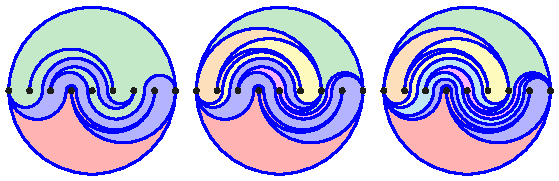
\includegraphics[scale=1.4]{wigglyPseudodissections}}
\caption{Three wiggly pseudodissections for~$n = 7$. The left one has three wiggly cells, of respective degrees $3$ (red), $8$ (green), and $4$ (blue). The other two have $7$ pseudotriangles, and are obtained from each other by a flip.}
\label{fig:pseudodissections}
\end{figure}
\end{definition}

\begin{definition}
\label{def:wigglyComplex}
The \defn{wiggly complex}~$\wigglyComplex_n$ is the simplicial complex of subsets of pairwise compatible internal wiggly arcs.
%In other words, it is the clique complex of the compatibility graph on internal wiggly arcs.

\begin{figure}
\centerline{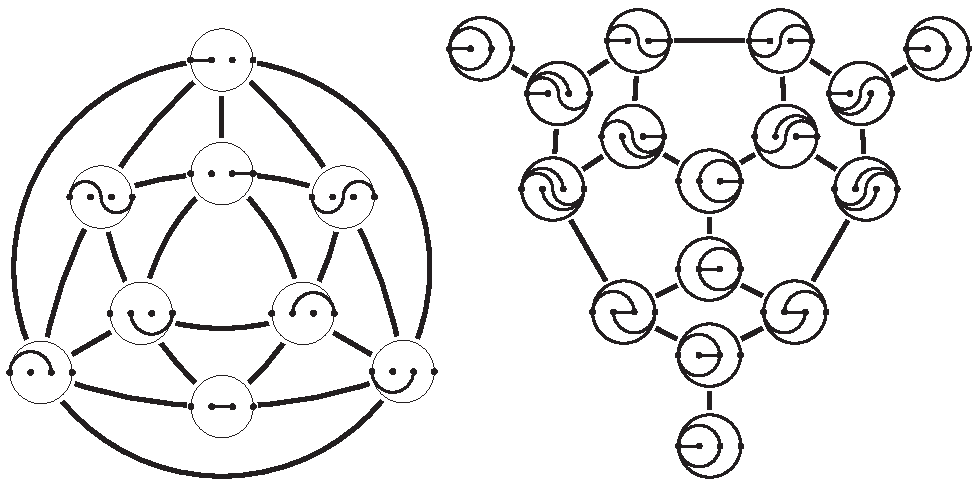
\includegraphics[scale=1.1]{wigglyComplex}}
\caption{The wiggly complex~$\wigglyComplex_2$ (left) and the wiggly flip graph~$\wigglyFlipGraph_2$ (right).}
\label{fig:wigglyComplex}
\end{figure}
\end{definition}

\begin{definition}
A wiggly pseudodissection~$D$ decomposes the digon bounded by~$\alpha_\mathrm{top}$ and~$\alpha_\mathrm{bot}$ into \defn{wiggly cells}.
The \defn{degree}~$\delta_c$ of a wiggly cell~$c$ is~$\delta_c \eqdef \beta_c/2+2\kappa_c-1$ where~$\beta_c$ is the number of wiggly arcs on the boundary of~$c$ (counted twice if they appear twice along the boundary of~$c$), and~$\kappa_c$ is the number of connected components of the boundary of~$c$.
Two consecutive wiggly arcs along the boundary of~$c$ define a \defn{corner} (resp.~a \defn{hinge}) of~$c$ if they bound a convex (resp.~concave) angle of~$c$.
%The \defn{concave chains} of~$c$ are the maximal sequences of wiggly arcs on the external boundary of~$c$ connected by hinges of~$c$.
\end{definition}

\begin{definition}
A \defn{wiggly pseudotriangle} (resp.~\defn{pseudoquadrangle}) is a cell of degree~$3$ (resp.~$4$).
\end{definition}

\begin{proposition}
\label{prop:wigglyPseudotriangulations}
Any wiggly pseudodissection~$D$ contains at most~$2n-1$ internal wiggly arcs and at most~$n$ wiggly cells.
Moreover, the following are equivalent:
\begin{compactenum}[(i)]
\item all wiggly cells of~$D$ are wiggly pseudotriangles,
\item $D$ contains~$n$ wiggly cells and is connected,
\item $D$ contains $2n-1$ internal wiggly arcs,
\item $D$ is an inclusion maximal wiggly pseudodissection.
\end{compactenum}
We then say that~$D$ is a \defn{wiggly pseudotriangulation}.
\end{proposition}

\begin{example}
\label{exm:allSmallWigglyPseudotriangulations}
For~$n = 1$, the $2$ wiggly pseudotriangulations of $3$ points are \smash{\raisebox{-.3cm}{
\includegraphics[scale=.85]{wigglyPseudotriangulation1}}} and \smash{\raisebox{-.3cm}{
\includegraphics[scale=.85]{wigglyPseudotriangulation2}}}.
For~${n = 2}$, the $14$ wiggly pseudotriangulations of $4$ points are \\[.2cm]
\centerline{
\includegraphics[scale=.85]{wigglyPseudotriangulations}}
\end{example}

%\begin{remark}
%\label{rem:numberWigglyPseudotriangulations}
%The number~$wp_n$ of wiggly pseudotriangulations of~$n+2$ points is given by
%\[
%\begin{array}{c|ccccccccc}
%n & 1 & 2 & 3 & 4 & 5 & 6 & 7 & 8 & \dots \\
%\hline
%wp_n & 2 & 14 & 176 & 3232 & 78384 & 2366248 & 85534176 & 3602770400 & \dots
%\end{array}
%\]
%To compute~$wp_n$, denote by $wp_n(x)$ the polynomial where the coefficient of~$x^i$ is the number of wiggly pseudotriangulations of~$n+2$ points with~$i$ \defn{final} internal wiggly arcs (\ie ending at the last point~$n+1$).
%For instance,
%\begin{align*}
%%	wp_0(x) & = 1, \\
%	wp_1(x) & = x + 1, \\
%	wp_2(x) & = 3 x^3 + 5 x^2 + 4 x + 2, \\
%	wp_3(x) & = 15 x^5 + 35 x^4 + 44 x^3 + 40 x^2 + 28 x + 14, \\
%	wp_4(x) & = 105 x^7 + 315 x^6 + 520 x^5 + 630 x^4 + 620 x^3 + 514 x^2 + 352 x + 176.
%\end{align*}
%We invite the reader to check the expressions of~$wp_1(x)$ and~$wp_2(x)$ with \cref{exm:allSmallWigglyPseudotriangulations}.
%We use this additional variable~$x$ to obtain a recursive formula for~$wp_n(x)$.
%%Indeed, any wiggly pseudotriangulation on~$n+1$ points can be obtained from a wiggly pseudotriangulation on~$n+2$ points by collapsing the points~$n$ and~$n+1$.
%Indeed, any wiggly pseudotriangulation of~$n+2$ points can be obtained from a wiggly pseudotriangulation of~$n+1$ points by inserting a single wiggly pseudotriangle with a hinge at~$n$.
%%There are two kinds of wiggly pseudotriangulations of~$n+2$ points:
%%\begin{itemize}
%%\item those with the wiggly arc~$(n, n+1, \varnothing, \varnothing)$ are obtained from a wiggly pseudotriangulation of~$n+1$ points by choosing the position of the only corner of~$t_n$ which is not at~$n+1$,
%%\item those without the wiggly arc~$(n, n+1, \varnothing, \varnothing)$ are obtained from a wiggly pseudotriangulation of~$n+1$ points by choosing the positions of the two corners of~$t_n$ which are not at~$n+1$.
%%\end{itemize}
%Each wiggly pseudotriangulation of~$n+1$ points with $i$ final internal wiggly arcs contributes to:
%\begin{compactitem}
%\item $i+2$ wiggly pseudotriangulations of~$n+2$ points with $i+2$ final internal wiggly arcs, containing the wiggly arc~$(n, n+1, \varnothing, \varnothing)$,
%\item $j+1$ wiggly pseudotriangulations of~$n+2$ points with $j$ final internal wiggly arcs, not containing the wiggly arc~$(n, n+1, \varnothing, \varnothing)$,  for all~$0 \le j \le i+1$.
%\end{compactitem}
%\pagebreak
%This translates to the recursive formula %for all~$n \ge 1$,
%\begin{align*}
%wp_{n}(x) & = \overbracket[.5pt]{x \cdot \frac{\partial}{\partial x} \big( x^2 wp_{n-1}(x) \big)}^{\substack{\text{wiggly pseudotriangulations} \\ \text{containing } (n, n+1, \varnothing, \varnothing)}} + \overbracket[.5pt]{\frac{\partial}{\partial x}\Big( \smash{\frac{wp_{n-1}(1)-x^3wp_{n-1}(x)}{1-x}} \Big)}^{\substack{\qquad\; \text{wiggly pseudotriangulations} \qquad\;  \\ \text{not containing } (n, n+1, \varnothing, \varnothing)}} \\
%& = \frac{1}{(1 - x)^2} \big( wp_{n-1}(1) + x^2 (2 x^2 - 2 x - 1) wp_{n-1}(x) + x^4 (x - 1) wp_{n-1}’(x) \big).
%\end{align*}
%This enables us to quickly compute~$wp_n(x)$ and we obtain the numbers of wiggly pseudotriangulations~$wp_n$ by evaluating~$wp_n(x)$ at~$x = 1$.
%\end{remark}

\begin{definition}
A \defn{wiggly diagonal} of a cell~$c$ is a wiggly arc inside~$c$ and compatible with~$c$.
\end{definition}

\begin{proposition}
\label{prop:diagonalsPseudoquadrangle}
Any wiggly pseudoquadrangle has exactly two wiggly diagonals.
Moreover, these two wiggly diagonals either cross precisely once, or are non pointed.
\end{proposition}

\begin{definition}
\label{def:wigglyFlipGraph}
The \defn{wiggly flip graph}~$\wigglyFlipGraph_n$ is the graph with a vertex for each wiggly pseudotriangulation, and with an edge between two wiggly pseudotriangulations~$T$ and~$T'$ if there are wiggly arcs~$\alpha \in T$ and~$\alpha' \in T'$ such that~$T \ssm \{\alpha\} = T' \ssm \{\alpha'\}$.
\end{definition}

Consider any wiggly arc~$\alpha$ in a wiggly pseudotriangulation~$T$.
By \cref{prop:diagonalsPseudoquadrangle}, the wiggly pseudoquadrangle formed by the union of the two wiggly pseudotriangles of~$T$ containing~$\alpha$ has two wiggly diagonals, $\alpha$ and another one~$\alpha'$.
Exchanging $\alpha$ by~$\alpha'$ gives a neighbor~$T'$ of~$T$ in the wiggly flip graph.
This leads to the following statement.

\begin{proposition}
\label{prop:wigglyFlipGraph}
The wiggly flip graph~$\wigglyFlipGraph_n$ is $(2n-1)$-regular and connected.
\end{proposition}

\cref{prop:wigglyPseudotriangulations,prop:wigglyFlipGraph} imply the main statement of this section.

\begin{theorem}
The wiggly complex~$\wigglyComplex_n$ is a flag $(2n-1)$-pseudomanifold without boundary.
\end{theorem}

Finally, we identify an important property of flips in wiggly pseudotriangulations.

\begin{proposition}
\label{prop:uerp}
Let~$\alpha \eqdef (i, j, A, B)$ and~$\alpha' \eqdef (i', j', A', B')$ be two exchangeable wiggly arcs.
Then any wiggly arc compatible with both~$\alpha$ and~$\alpha'$ is also compatible with the wiggly~arcs:
\begin{compactitem}
\item $\beta \eqdef (i, j', A \cup A', B \cup B' \cup \{j\})$ and~$\beta' \eqdef (i, j', A \cup A' \cup \{j\}, B \cup B')$ if~$\alpha$ and~$\alpha'$ are non pointed with~$j = i'$,
(In other words, ~$\beta$ and~$\beta'$ are the two wiggly arcs starting at~$\min(i,i')$ and ending at~$\max(j,j')$ which follow $\alpha$ on~$]i,j[$ and~$\alpha'$ on~$]i',j'[$.)
\item $\beta \!\eqdef\! \big( i, j', {]i,j'[} \!\ssm\! (B \!\cup\! B'), {]i,j'[} \!\cap\! (B \!\cup\! B') \big)$ and~$\beta' \!\eqdef\! \big( i', j, {]i',j[} \!\cap\! (A \!\cup\! A'), {]i',j[} \!\ssm\! (A \!\cup\! A') \big)$ if~$\alpha$ and~$\alpha'$ are crossing and there is~$k \in [n-1]$ with~$k \in (A \cap B') \cup (\{i\} \cap B') \cup (A \cap \{i'\})$ and~$k+1 \in (A' \cap B) \cup (\{j'\} \cap B) \cup (A' \cap \{j\})$.
(In other words, $\beta$ is the wiggly arc starting at~$i$ and ending at~$j'$ which follows the lower hull of~$\alpha$ and~$\alpha'$, and~$\beta'$ is the wiggly arc starting at~$i'$ and ending~at~$j$ which follows the upper hull of~$\alpha$ and~$\alpha'$.)
\end{compactitem}
%See \cref{fig:incompatible3} for illustrations.
%(By exchanging~$\alpha$ and~$\alpha'$, similar statements hold if~$\alpha$ and~$\alpha'$ are non pointed with~$j = i'$, or if~$\alpha$ and~$\alpha'$ are crossing with~$i \in B'$ or~$i' \in A$.)
%
%\begin{figure}

%\vspace{-.1cm}
\centerline{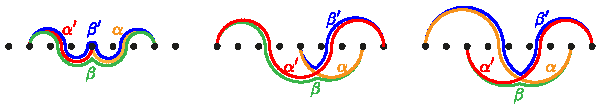
\includegraphics[scale=1.3]{incompatible3}}
%\caption{The wiggly arcs~$\beta$ and~$\beta'$ of \cref{prop:uerp}.}
%\label{fig:incompatible3}
%\end{figure}
\vspace{-.4cm}
\end{proposition}

\section{Wiggly permutations and the wiggly lattice}
\label{sec:wigglyPermutations}

We now define the wiggly lattice on wiggly permutations of~$[2n]$, illustrated in \cref{fig:wigglyLattice}.

\begin{definition}
\label{def:wigglyPermutation}
A \defn{wiggly permutation} is a permutation of~$[2n]$ which avoids the patterns:
\begin{compactitem}
\item $(2j-1) \cdots i \cdots (2j)$ for~$j \in [n]$ and~$i < 2j-1$,
\item $(2j) \cdots k \cdots (2j-1)$ for~$j \in [n]$ and~$k > 2j$.
\end{compactitem}
\end{definition}

\begin{example}
\label{exm:allSmallWigglyPermutations}
For~$n = 1$, the $2$ wiggly permutations of~$[2]$ are~$12$ and~$21$.
For~$n = 2$, the $14$ wiggly permutations of~$[4]$ are
\vspace{-.1cm}
\[
1234, 1243, 1342, 1423, 1432, 2134, 2143, 3412, 3421, 4123, 4132, 4213, 4312, 4321.
\]
%The wiggly permutations of~$[6]$ are
%\begin{gather*}
%123456, 213456, 134256, 124356, 123564, 123465, 342156, 214356, 213564, 213465, 341256, 143256, \\
%134562, 134265, 142356, 125643, 124365, 135642, 125634, 123654, 123645, 432156, 345621, 342165, \\
%421356, 215643, 214365, 356421, 215634, 213654, 213645, 431256, 341562, 341265, 413256, 143562, \\
%143265, 134652, 134625, 412356, 156423, 142365, 156243, 126543, 126435, 356412, 156342, 136542, \\
%156234, 126534, 126354, 136425, 126345, 435621, 432165, 346521, 346215, 564213, 421365, 562143, \\
%216543, 216435, 563421, 365421, 562134, 216534, 216354, 364215, 216345, 431562, 431265, 345612, \\
%341652, 341625, 413562, 413265, 156432, 143652, 143625, 136452, 564123, 412365, 561423, 165423, \\
%164235, 561243, 165243, 162543, 162435, 563412, 365412, 561342, 165342, 163542, 561234, 165234, \\
%162534, 162354, 364125, 163425, 162345, 564321, 436521, 436215, 364521, 654213, 642135, 652143, \\
%621543, 621435, 653421, 635421, 652134, 621534, 621354, 634215, 621345, 435612, 431652, 431625, \\
%346512, 346152, 346125, 564132, 413652, 413625, 561432, 165432, 164352, 164325, 364152, 163452, \\
%654123, 641235, 651423, 615423, 614235, 651243, 615243, 612543, 612435, 653412, 564312, 635412, \\
%651342, 615342, 613542, 651234, 615234, 612534, 612354, 634125, 613425, 612345, 654321, 643521, \\
%643215, 634521, 436512, 436152, 436125, 364512, 654132, 641352, 641325, 651432, 615432, 614352, \\
%614325, 634152, 613452, 654312, 643125, 643512, 643152, 634512.
%\end{gather*}
\end{example}

\begin{proposition}
The wiggly permutations induce a sublattice of the weak order on permutations of~$[2n]$, that we call the \defn{wiggly lattice}~$\wigglyLattice_n$.
\end{proposition}

\begin{proposition}
Any wiggly permutation covers (resp.~is covered by) one wiggly permutation~for each of its descents (resp.~ascents).
The cover graph of~$\wigglyLattice_n$ is $(2n-1)$-regular~and~connected.
\end{proposition}

%\begin{remark}
%\label{rem:numberWigglyPermutations}
%The number~$wp_n$ of wiggly permutations of~$[2n]$ is given by
%\[
%\begin{array}{c|ccccccccc}
%n & 1 & 2 & 3 & 4 & 5 & 6 & 7 & 8 & \dots \\
%\hline
%wp_n & 2 & 14 & 176 & 3232 & 78384 & 2366248 & 85534176 & 3602770400 & \dots
%\end{array}
%\]
%To compute~$wp_n$, denote by $wp_n(x)$ the polynomial where the coefficient of~$x^i$ is the number of wiggly permutations of~$[2n]$ with $i$ \defn{admissible gaps} (\ie gaps~$\gamma$ between two consecutive positions such that there is no~$j \in [n]$ such that the value~$2j$ appears before the gap~$\gamma$ while the value~$2j-1$ appears after the gap~$\gamma$).
%For instance,
%\begin{align*}
%%	wp_0(x) & = 1, \\
%	wp_1(x) & = x + 1, \\
%	wp_2(x) & = 3 x^3 + 5 x^2 + 4 x + 2, \\
%	wp_3(x) & = 15 x^5 + 35 x^4 + 44 x^3 + 40 x^2 + 28 x + 14. % \\
%%	wp_4(x) & = 105 x^7 + 315 x^6 + 520 x^5 + 630 x^4 + 620 x^3 + 514 x^2 + 352 x + 176.
%\end{align*}
%%We invite the reader to check the expressions of~$wp_1(x)$ and~$wp_2(x)$ with \cref{exm:allSmallWigglyPermutations}.
%Any wiggly permutation of~$[2n]$ can be obtained from a wiggly permutation of~$[2n-2]$ by inserting the last values~$2n-1$ and~$2n$.
%Each wiggly permutation of~$[2n-2]$ with $i$ admissible gaps contributes to:
%\begin{compactitem}
%\item $i+2$ wiggly permutations of~$[2n]$ with $i+2$ admissible gaps and where~$2n-1$ appears before~$2n$ (they must appear consecutively),
%\item $j+1$ wiggly permutations of~$[2n]$ with $j$ admissible arcs and where $2n$ appears before~$2n-1$, for all~$0 \le j \le i+1$.
%\end{compactitem}
%%We thus obtain the same recursive equation on~$wp_n(x)$ as in \cref{rem:numberWigglyPseudotriangulations}.
%This translates to the recursive formula %for all~$n \ge 1$,
%\begin{align*}
%wp_{n}(x) & = \overbracket[.5pt]{x \cdot \frac{\partial}{\partial x} \big( x^2 wp_{n-1}(x) \big)}^{\substack{\text{wiggly permutations} \\ \text{with~$2n-1$ before~$2n$}}} + \overbracket[.5pt]{\frac{\partial}{\partial x}\Big( \smash{\frac{wp_{n-1}(1)-x^3wp_{n-1}(x)}{1-x}} \Big)}^{\substack{\qquad\; \text{wiggly permutations} \qquad\;  \\ \text{with~$2n$ before~$2n-1$}}} \\
%& = \frac{1}{(1 - x)^2} \big( wp_{n-1}(1) + x^2 (2 x^2 - 2 x - 1) wp_{n-1}(x) + x^4 (x - 1) wp_{n-1}’(x) \big).
%\end{align*}
%This enables us to quickly compute~$wp_n(x)$ and we obtain the numbers of wiggly pseudotriangulations~$wp_n$ by evaluating~$wp_n(x)$ at~$x = 1$.
%\end{remark}

\newpage
\section{Bijection}
\label{sec:bijection}

\begin{figure}[t]
\centerline{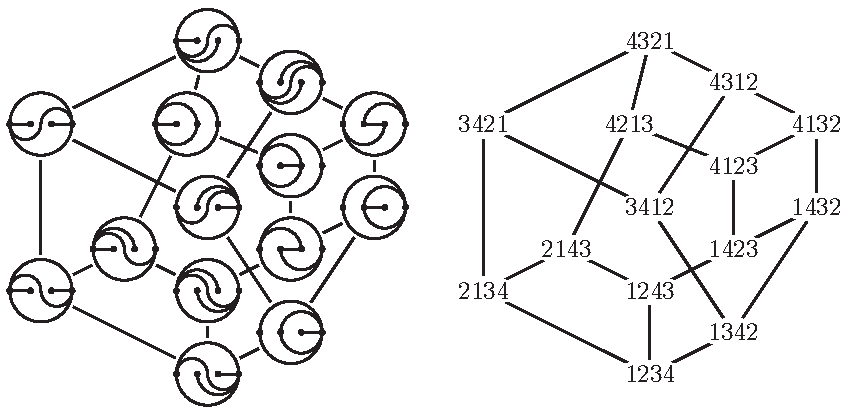
\includegraphics[scale=1.1]{wigglyLattice}}
\caption{The wiggly lattice~$\wigglyLattice_2$ on wiggly pseudotriangulations (left) and on wiggly permutations (right).}
\label{fig:wigglyLattice}
\end{figure}

We now prove that wiggly pseudotriangulations and wiggly permutations are in bijection.
%, and that this bijection induces an isomorphism from the wiggly flip graph to the cover graph of the wiggly lattice.
The following two definitions are illustrated in \cref{fig:wigglyLattice}.

%\begin{figure}
%\centerline{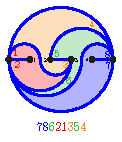
\includegraphics[scale=1.7]{bijection}}
%\caption{The bijection between wiggly pseudotriangulations and wiggly permutations.}
%\label{fig:bijection}
%\end{figure}

\parpic(3.6cm,5cm)(-10pt, 133pt)[r][b]{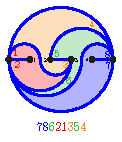
\includegraphics[scale=2]{bijection}}{
\begin{definition}
\label{def:bijection1}
Consider a wiggly pseudotriangulation~$T$.
Rotating counterclockwise inside each wiggly pseudotriangle of~$T$, we label by~$2h-1$ (resp.~$2h+1$) the corner immediately preceding (resp.~following) the hinge~$h$ (the remaining corner remains unlabelled).
Define~$\Phi(T)$ as the permutation obtained by reading these labels from bottom to top, meaning that for each internal wiggly arc~$\alpha$ of~$T$, the label incident to~$\alpha$ and below~$\alpha$ appears just before the label incident to~$\alpha$ and above~$\alpha$.
See example on the right.
\end{definition}

\begin{definition}
\label{def:bijection2}
For a wiggly permutation~$\sigma$ of~$[2n]$, define~$\Psi(\sigma) \eqdef \set{\alpha(\sigma, k)}{k \in [2n-1]}$, where for~$k \in [2n-1]$, we have~$\alpha(\sigma, k) \eqdef ( i, j, A, B)$ with
\begin{alignat*}{3}
i & \eqdef \max \{0\} \cup \set{i \!\in\! [n]}{2i-1 \!\in\! \sigma([k]) \!\!\not\ni\! 2i}\!, \quad &
A & \eqdef \set{\ell \!\in\! {]i,j[}}{\{2\ell-1, 2\ell\} \!\subseteq\! \sigma([k])}\!, \\
j & \eqdef \min \{n+1\} \cup \set{j \!\in\! [n]}{2j \!\in\! \sigma([k]) \!\!\not\ni\! 2j-1}\!, \;\, &
B & \eqdef \set{\ell \!\in\! {]i,j[}}{\{2\ell-1, 2\ell\} \cap \sigma([k]) \!=\! \varnothing} \!.
\end{alignat*}
\end{definition}
}

\begin{proposition}
\label{prop:bijection}
The maps~$\Phi$ of \cref{def:bijection1} and $\Psi$ of \cref{def:bijection2} define inverse bijections between the wiggly pseudotriangulations and the wiggly permutations, inducing a graph isomorphism between the wiggly flip graph~$\wigglyIncreasingFlipGraph_n$ and the cover diagram of the wiggly lattice~$\wigglyLattice_n$.
\end{proposition}

\newpage
\section{Wiggly fan}
\label{sec:wigglyFan}

We denote by~$\smash{(\b{e}_i)_{i \in [d]}}$ the standard basis of~$\R^d$.
For~$I \subseteq [d]$, we define~$\one_I \eqdef \sum_{i \in I} \b{e}_i$, and we often shorten~$\smash{\one_{[d]}}$ by~$\one_d$.
We denote by~$\HH_d$ the hyperplane of~$\R^d$ defined by the equation~$\dotprod{\b{x}}{\one_d} = 0$, and we denote by~$\pi : \R^d \to \HH$ the orthogonal projection on~$\HH_d$, that is~$\pi(\b{x}) \eqdef \b{x} - (\dotprod{\b{x}}{\one_d} / d) \one_d$.
%
We now define a first family of vectors, see \cref{fig:pseudotriangulationMatrices}.
%
\begin{figure}[b]
\centerline{\raisebox{-1.8cm}{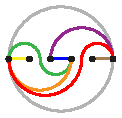
\includegraphics[scale=2]{pseudotriangulationMatrices}} \quad \scalebox{.9}{
\(
\begin{blockarray}{ccccccccc}
	& & {\color{brown} \bullet} & {\color{red} \bullet} & {\color{orange} \bullet} & {\color{yellow} \bullet} & {\color{green} \bullet} & {\color{blue} \bullet} & {\color{violet} \bullet} \\
	\begin{block}{c@{\hspace*{-.1cm}}c(ccccccc)}
	1 & & 0 & \!\! -1 \!\! & \!\! -1 \!\! & \!\! -1 \!\! & 1 & 0 & 0 \\
	2 & & 0 & \!\! -1 \!\! & \!\! -1 \!\! & 1 & 1 & 0 & 0 \\
	3 & & 0 & \!\! -1 \!\! & \!\! -1 \!\! & 0 & \!\! -1 \!\! & 1 & 1 \\
	4 & & 0 & \!\! -1 \!\! & \!\! -1 \!\! & 0 & \!\! -1 \!\! & \!\! -1 \!\! & \!\!\! -1 \! \\
	5 & & 0 & \!\! -1 \!\! & \!\! -1 \!\! & 0 & \!\! -1 \!\! & \!\! -1 \!\! & 1 \\
	6 & & 0 & \!\! -1 \!\! & 1 & 0 & 1 & 1 & 1 \\
	7 & & 1 & 1 & 0 & 0 & 0 & 0 & 1 \\
	8 & & \! -1 \!\!\! & 1 & 0 & 0 & 0 & 0 & 1 \\
	\end{block}
	& & & & \multicolumn{2}{c}{$\hat{\b{g}}(T)$} & &
\end{blockarray}
%
\qquad
%
\begin{blockarray}{ccccccccc}
	& & {\color{brown} \bullet} & {\color{red} \bullet} & {\color{orange} \bullet} & {\color{yellow} \bullet} & {\color{green} \bullet} & {\color{blue} \bullet} & {\color{violet} \bullet} \\
	\begin{block}{c@{\hspace*{-.1cm}}c(ccccccc)}
	1 & & 0 & 0 & \!\! -1 \!\! & 2 & 1 & 0 & 0 \\
	2 & & 0 & 0 & \!\! -1 \!\! & \!\! -2 \!\! & 1 & 0 & 0 \\
	3 & & 0 & 0 & \!\! -1 \!\! & 0 & \!\! -1 \!\! & 2 & 0 \\
	4 & & 0 & 0 & 1 & 0 & \!\! -1 \!\! & 0 & \!\! -2 \!\! \\
	5 & & 0 & \!\! -1 \!\! & 0 & 0 & 0 & \!\! -2 \!\! & 2 \\
	6 & & 0 & \!\! -1 \!\! & 2 & 0 & 0 & 0 & 0 \\
	7 & & 2 & 1 & 0 & 0 & 0 & 0 & 0 \\
	8 & & \! -2 \!\!\! & 1 & 0 & 0 & 0 & 0 & 0 \\
	\end{block}
	& & & & \multicolumn{2}{c}{$4\b{c}(T)$} & &
\end{blockarray}
\)
}}
\caption{The $\b{g}$-matrix~$\b{g}(T)$ and $\b{c}$-matrix~$\b{c}(T)$ of a wiggly pseudotriangulation~$T$.} % The $i$th column of these matrices are the $\b{g}$-vector~$\b{g}(\alpha)$ and $4$ times the $\b{c}$-vector~$\b{c}(\alpha, T)$ of the $i$th wiggly arc~$\alpha$ of~$T$ (ordered from bottom to top). The colors of the columns match the colors of the wiggly arcs.}
\label{fig:pseudotriangulationMatrices}
\end{figure}

\begin{definition}
\label{def:gvectors}
The \defn{$\b{g}$-vector}~$\b{g}(\alpha)$ of a wiggly arc~$\alpha \eqdef (i, j, A, B)$ is defined as the projection~$\pi \big( \hat{\b{g}}(\alpha) \big)$ of the vector~$\hat{\b{g}}(\alpha) \eqdef \one_{\alpha^+} - \one_{\alpha^-}$ where
\vspace{-.25cm}
\begin{align*}
\alpha^+ & \eqdef \big(\{2i-1, 2j\} \ssm \{-1, 2n+2\} \big) \cup \set{2a-1}{a \in A} \cup \set{2a}{a \in A},
\\
\alpha^- & \eqdef \big(\{2i, 2j-1\} \ssm \{0, 2n+1\} \big) \cup \set{2b-1}{b \in B} \cup \set{2b}{b \in B}.
\\[-.9cm]
\end{align*}
%If we place the coordinate~$2p-1$ on the left and the coordinate~$2p$ on the right of point~$p$, then~$\b{g}(\alpha)$ has a $1$ outside its two endpoints and on both sides of points in~$A$, and a~$-1$ inside its two endpoints and on both sides of points in~$B$.
%Note that ${\hat{\b{g}} \big( (0, n+1, [n], \varnothing) \big) = \one_{2n} = - \hat{\b{g}} \big( (0, n+1, \varnothing, [n]) \big)}$, so that~${\b{g} \big( (0, n+1, [n], \varnothing) \big) = \b{0} = \b{g} \big( (0, n+1, \varnothing, [n]) \big)}$.
\noindent
We define~$\b{g}(D) \eqdef \set{\b{g}(\alpha)}{\alpha \in D^\circ}$ for a set~$D$ of wiggly arcs.
\end{definition}

The main feature of these $\b{g}$-vectors is that we control their behavior under flip.

\begin{proposition}
\label{prop:linearDependences}
Let~$T$ and~$T'$ be two wiggly pseudotriangulations with~$T \ssm \{\alpha\} = T' \ssm \{\alpha'\}$, and let~$\beta$ and~$\beta'$ be the wiggly arcs defined in \cref{prop:uerp}.
Then~$\{\beta, \beta'\} \in T \cap T'$ and
\begin{compactitem}
\item if $\alpha$ and~$\alpha'$ are not pointed, then~$\b{g}(\alpha) + \b{g}(\alpha') = \big( \b{g}(\beta) + \b{g}(\beta') \big) / 2$,
\item if~$\alpha$ and~$\alpha'$ are crossing, then~${\b{g}(\alpha) + \b{g}(\alpha') = \b{g}(\beta) + \b{g}(\beta')}$.
\end{compactitem}
\end{proposition}

This property implies in particular that the $\b{g}$-vectors of each wiggly pseudotriangulation form a basis of~$\HH_{2n}$, which enables us to define the dual basis, called $\b{c}$-vectors.

\begin{proposition}
\label{prop:basis}
For any wiggly pseudotriangulation~$T$, the set~$\b{g}(T)$ is a basis of~$\HH_{2n}$.
\end{proposition}

\begin{definition}
\label{def:cvectors}
The \defn{$\b{c}$-vector} of an interior wiggly arc~$\alpha$ in a \mbox{wiggly pseudotriangulation~$T$} is the vector~$\b{c}(\alpha, T)$ of~$\HH_{2n}$ such that~$\dotprod{\b{c}(\alpha, T)\!}{\!\b{g}(\alpha)} \!=\! 1$ and~$\dotprod{\b{c}(\alpha, T)\!}{\!\b{g}(\alpha')} \!=\! 0$~for~all wiggly arcs~$\alpha' \ne \alpha$ of~$T$.
That is, $\b{c}(T) \eqdef \! \set{\b{c}(\alpha, T)}{\alpha \in T^\circ}$ and~$\b{g}(T)$ are dual bases~in~$\HH_{2n}$.
\end{definition}

We finally exploit $\b{g}$-vectors to support the wiggly fan realizing the wiggly complex.

\begin{theorem}
\label{thm:wigglyFan}
The collection of cones~$\R_{\ge 0} \b{g}(D) $ for all wiggly dissections~$D$ in the wiggly complex~$\wigglyComplex_n$ forms a complete simplicial fan of~$\HH_{2n}$, called the \defn{wiggly fan}~$\wigglyFan_n$.
\end{theorem}

\newpage
\section{Wigglyhedron}
\label{sec:wigglyhedron}

We now construct the wigglyhedron illustrated in \cref{fig:wigglyhedron} when~${n = 2}$.
For this, we just choose a support function on the rays of the wiggly fan~$\wigglyFan_n$, inspired from~\cite{HohlwegPilaudStella,PaluPilaudPlamondon-nonkissing}.
%
\begin{figure}[b]
\centerline{\begin{tikzpicture}%
	[x={(0.681462cm, -0.327528cm)},
	y={(0.731633cm, 0.326817cm)},
	z={(-0.017949cm, 0.886519cm)},
	scale=.500000,
	back/.style={color=blue, thin},
	edge/.style={color=blue, very thick, },
	facet/.style={fill=blue,fill opacity=0.00000},
	vertex/.style={inner sep=1pt,circle,draw=blue,fill=blue,thick}]
%
%
%% This TikZ-picture was produce with Sagemath version 9.5
%% with the command: ._tikz_3d_in_3d and parameters:
%% view = [-764, -346, -545]
%% angle = 76.39
%% scale = 1
%% edge_color = blue
%% facet_color = blue
%% opacity = 0.5
%% vertex_color = blue
%% axis = False

%% Coordinate of the vertices:
%%
\coordinate (-1.00000, -4.00000, -3.00000) at (-1.00000, -4.00000, -3.00000);
\coordinate (1.00000, 0.00000, -3.00000) at (1.00000, 0.00000, -3.00000);
\coordinate (3.00000, 4.00000, 1.00000) at (3.00000, 4.00000, 1.00000);
\coordinate (3.00000, 2.00000, -1.00000) at (3.00000, 2.00000, -1.00000);
\coordinate (3.00000, 0.00000, -1.00000) at (3.00000, 0.00000, -1.00000);
\coordinate (1.00000, -2.00000, -3.00000) at (1.00000, -2.00000, -3.00000);
\coordinate (3.00000, 4.00000, 5.00000) at (3.00000, 4.00000, 5.00000);
\coordinate (3.00000, 0.00000, 3.00000) at (3.00000, 0.00000, 3.00000);
\coordinate (-1.00000, -4.00000, 1.00000) at (-1.00000, -4.00000, 1.00000);
\coordinate (-5.00000, -4.00000, 1.00000) at (-5.00000, -4.00000, 1.00000);
\coordinate (-5.00000, -4.00000, -3.00000) at (-5.00000, -4.00000, -3.00000);
\coordinate (-3.00000, 0.00000, -3.00000) at (-3.00000, 0.00000, -3.00000);
\coordinate (-1.00000, 4.00000, 1.00000) at (-1.00000, 4.00000, 1.00000);
\coordinate (-1.00000, 4.00000, 5.00000) at (-1.00000, 4.00000, 5.00000);
%%
%%
%% Drawing edges in the back
%%
\draw[edge,back] (1.00000, 0.00000, -3.00000) -- (-3.00000, 0.00000, -3.00000);
\draw[edge,back] (3.00000, 4.00000, 1.00000) -- (-1.00000, 4.00000, 1.00000);
\draw[edge,back] (-5.00000, -4.00000, -3.00000) -- (-3.00000, 0.00000, -3.00000);
\draw[edge,back] (-3.00000, 0.00000, -3.00000) -- (-1.00000, 4.00000, 1.00000);
\draw[edge,back] (-1.00000, 4.00000, 1.00000) -- (-1.00000, 4.00000, 5.00000);
%%
%%
%% Drawing vertices in the back
%%
\node[vertex] at (-1.00000, 4.00000, 1.00000)     {};
\node[vertex] at (-3.00000, 0.00000, -3.00000)     {};
%%
%%
%% Drawing the facets
%%
\fill[facet] (3.00000, 0.00000, 3.00000) -- (3.00000, 0.00000, -1.00000) -- (3.00000, 2.00000, -1.00000) -- (3.00000, 4.00000, 1.00000) -- (3.00000, 4.00000, 5.00000) -- cycle {};
\fill[facet] (1.00000, -2.00000, -3.00000) -- (1.00000, 0.00000, -3.00000) -- (3.00000, 2.00000, -1.00000) -- (3.00000, 0.00000, -1.00000) -- cycle {};
\fill[facet] (-1.00000, -4.00000, 1.00000) -- (-1.00000, -4.00000, -3.00000) -- (1.00000, -2.00000, -3.00000) -- (3.00000, 0.00000, -1.00000) -- (3.00000, 0.00000, 3.00000) -- cycle {};
\fill[facet] (-1.00000, 4.00000, 5.00000) -- (3.00000, 4.00000, 5.00000) -- (3.00000, 0.00000, 3.00000) -- (-1.00000, -4.00000, 1.00000) -- (-5.00000, -4.00000, 1.00000) -- cycle {};
\fill[facet] (-5.00000, -4.00000, -3.00000) -- (-1.00000, -4.00000, -3.00000) -- (-1.00000, -4.00000, 1.00000) -- (-5.00000, -4.00000, 1.00000) -- cycle {};
%%
%%
%% Drawing edges in the front
%%
\draw[edge] (-1.00000, -4.00000, -3.00000) -- (1.00000, -2.00000, -3.00000);
\draw[edge] (-1.00000, -4.00000, -3.00000) -- (-1.00000, -4.00000, 1.00000);
\draw[edge] (-1.00000, -4.00000, -3.00000) -- (-5.00000, -4.00000, -3.00000);
\draw[edge] (1.00000, 0.00000, -3.00000) -- (3.00000, 2.00000, -1.00000);
\draw[edge] (1.00000, 0.00000, -3.00000) -- (1.00000, -2.00000, -3.00000);
\draw[edge] (3.00000, 4.00000, 1.00000) -- (3.00000, 2.00000, -1.00000);
\draw[edge] (3.00000, 4.00000, 1.00000) -- (3.00000, 4.00000, 5.00000);
\draw[edge] (3.00000, 2.00000, -1.00000) -- (3.00000, 0.00000, -1.00000);
\draw[edge] (3.00000, 0.00000, -1.00000) -- (1.00000, -2.00000, -3.00000);
\draw[edge] (3.00000, 0.00000, -1.00000) -- (3.00000, 0.00000, 3.00000);
\draw[edge] (3.00000, 4.00000, 5.00000) -- (3.00000, 0.00000, 3.00000);
\draw[edge] (3.00000, 4.00000, 5.00000) -- (-1.00000, 4.00000, 5.00000);
\draw[edge] (3.00000, 0.00000, 3.00000) -- (-1.00000, -4.00000, 1.00000);
\draw[edge] (-1.00000, -4.00000, 1.00000) -- (-5.00000, -4.00000, 1.00000);
\draw[edge] (-5.00000, -4.00000, 1.00000) -- (-5.00000, -4.00000, -3.00000);
\draw[edge] (-5.00000, -4.00000, 1.00000) -- (-1.00000, 4.00000, 5.00000);
%%
%%
%% Drawing the vertices in the front
%%
\node[vertex] at (-1.00000, -4.00000, -3.00000)     {};
\node[vertex] at (1.00000, 0.00000, -3.00000)     {};
\node[vertex] at (3.00000, 4.00000, 1.00000)     {};
\node[vertex] at (3.00000, 2.00000, -1.00000)     {};
\node[vertex] at (3.00000, 0.00000, -1.00000)     {};
\node[vertex] at (1.00000, -2.00000, -3.00000)     {};
\node[vertex] at (3.00000, 4.00000, 5.00000)     {};
\node[vertex] at (3.00000, 0.00000, 3.00000)     {};
\node[vertex] at (-1.00000, -4.00000, 1.00000)     {};
\node[vertex] at (-5.00000, -4.00000, 1.00000)     {};
\node[vertex] at (-5.00000, -4.00000, -3.00000)     {};
\node[vertex] at (-1.00000, 4.00000, 5.00000)     {};
%%
%%
\end{tikzpicture}}
\caption{The wigglyhedron~$\wigglyhedron_2$.}
\label{fig:wigglyhedron}
\end{figure}

\begin{definition}
\label{def:incompatibilityDegree}
The \defn{incompatibility degree}~$\delta(\alpha, \alpha')$ of~$\alpha \eqdef (i, j, A, B)$ and~$\alpha' \eqdef (i', j', A', B')$ is %given by
\begin{compactitem}
\item $0$ if~$\alpha$ and~$\alpha'$ are pointed and non-crossing,
\item $1$ is~$\alpha$ and~$\alpha'$ are not pointed, % (\ie $i = j'$ or~$i' = j$),
\item the number of crossings of~$\alpha$ and~$\alpha'$ if they are crossing. % (\ie the number of~$p \in \{0, \dots, n\}$ with $p \in (A \cap B') \cup (\{i,j\} \cap B') \cup (A \cap \{i',j'\})$ and~$p+1 \in (A' \cap B) \cup (\{i',j'\} \cap B) \cup (A' \cap \{i,j\})$, or the opposite).
\end{compactitem}
The \defn{incompatibility number} of a wiggly arc~$\alpha$ is~$\kappa(\alpha) \eqdef \sum_{\alpha'} \delta(\alpha, \alpha')$.
\end{definition}

Note that~$\delta(\alpha, \alpha')$ is indeed an incompatibility degree, in the sense that~$\alpha$ and~$\alpha'$ are compatible if and only if~$\delta(\alpha, \alpha') = 0$ and exchangeable if and only if~$\delta(\alpha, \alpha') = 1$.
The following statement is the main feature of the incompatibility number.

\begin{proposition}
\label{prop:wallCrossingInequalities}
Let~$T$ and~$T'$ be two wiggly pseudotriangulations with~$T \ssm \{\alpha\} = T' \ssm \{\alpha'\}$, and let~$\beta$ and~$\beta'$ be the wiggly arcs defined in \cref{prop:uerp}.
Then
\begin{compactitem}
\item if $\alpha$ and~$\alpha'$ are not pointed, then~$\kappa(\alpha) + \kappa(\alpha') > \big( \kappa(\beta) + \kappa(\beta') \big) / 2$,
\item if~$\alpha$ and~$\alpha'$ are crossing, then~${\kappa(\alpha) + \kappa(\alpha') > \kappa(\beta) + \kappa(\beta')}$.
\end{compactitem}
\end{proposition}

Combining \cref{prop:linearDependences,prop:wallCrossingInequalities}, the incompatibility number satisfies all wall-crossing inequalities of the wiggly fan~$\wigglyFan_n$, from which we derive our main statement.
%that it behaves properly with respect to the linear dependences of 

\begin{theorem}
\label{thm:wigglyhedron}
The wiggly fan~$\wigglyFan_n$ is the normal fan of a simplicial $(2n-1)$-dimensional polytope, called the \defn{wigglyhedron}~$\wigglyhedron_n$, and defined equivalently~as
\begin{compactitem}
\item the intersection of the halfspaces~$\set{\b{x} \!\in\! \HH_{2n}\!\!}{\!\!\dotprod{\b{g}(\alpha)\!}{\!\b{x}} \! \le \! \kappa(\alpha)}$ for all internal wiggly~arcs~$\alpha$,
\item the convex hull of the points~$\smash{\b{p}(T) \eqdef \!\! \displaystyle\sum\limits_{\alpha \in T} \!\kappa(\alpha) \, \b{c}(\alpha, T)}$ for all wiggly pseudotriangulations~$T$.
\end{compactitem}
\end{theorem}

\begin{proposition}
The Hasse diagram of the wiggly lattice~$\wigglyLattice_n$ is isomorphic to the graph of the wigglyhedron~$\wigglyhedron_n$ oriented in the direction
\(
\b{\omega} \eqdef \sum_{i \in [n]} 4ni (\b{e}_{2i-1} + \b{e}_{2i}) + \sum_{j \in [2n]} j \b{e}_j.
\)
\end{proposition}


\newpage
\section{Cambrian considerations}
\label{sec:CambrianConsiderations}

In this section, we fix a signature~$\delta \eqdef \delta_1 \dots \delta_n \in \{+,-\}^n$. By convention, $\delta_0 = \delta_{n+1} = 0$.
We connect the $\delta$-Cambrian lattice~\cite{Reading-CambrianLattices} to the wiggly lattice % of \cref{sec:wigglyPermutations} 
and the $\delta$-associahedron of~\cite{HohlwegLange} to the wigglyhedron. % of \cref{sec:wigglyhedron}.
\cref{def:CambrianTriangulations,def:CambrianPermutations,def:CambrianWigglyPseudotriangulations,def:CambrianWigglyPermutations,prop:CambrianLattice} are illustrated in \cref{fig:wigglyCambrian}.

\begin{figure}[b]
%\centerline{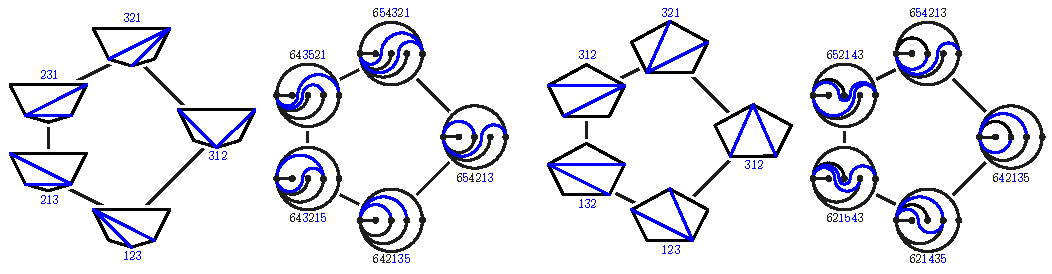
\includegraphics[scale=1]{wigglyCambrian1}}
%\vspace{-.3cm}
%\centerline{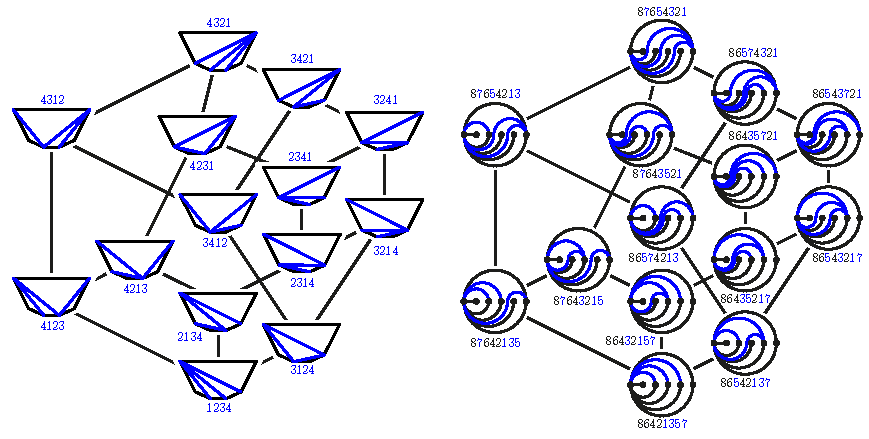
\includegraphics[scale=1.1]{wigglyCambrian2}}
%\vspace{-.5cm}
\centerline{\begin{overpic}[scale=.87]{wigglyCambrian3} \put(44,2){$\delta = {+}{+}{-}{-}$}\end{overpic}}
\caption{The $\delta$-Cambrian lattice (left) is an interval of the wiggly lattice~$\wigglyLattice_4$~(right).}
\label{fig:wigglyCambrian}
\end{figure}

\begin{definition}
\label{def:CambrianTriangulations}
The \defn{$\delta$-gon} is a convex $(n+2)$-gon with a point at abscissa~$i$ and ordinate of the same sign as~$\delta_i$  for~$0 \!\le\! i \!\le\! n+1$.
A \defn{$\delta$-triangulation} is a triangulation of the $\delta$-gon.
The \defn{$\delta$-triangulation lattice} is the transitive closure of slope increasing flips on $\delta$-triangulations.
%If~$T$ and~$T'$ are two $\delta$-triangulations with~$T \ssm \{d\} = T' \ssm \{d'\}$, then the flip from~$T$ to~$T'$ is \defn{increasing} if the slope of~$d$ is smaller than the slope of~$d'$.
\end{definition}

\begin{definition}
\label{def:CambrianPermutations}
A \defn{$\delta$-permutation} is a permutation of~$[n]$ avoiding $\cdots ik \cdots j \cdots$ if~$\delta_j = -$, and~$\cdots j \cdots ki \cdots$ if~$\delta_j = +$ for~$i < j < k$.
The \defn{$\delta$-permutation lattice} is the sublattice of the weak order induced by $\delta$-permutations.
\end{definition}

\begin{definition}
\label{def:CambrianWigglyPseudotriangulations}
The \defn{$\delta$-wiggly arcs} are the arcs~$(0, j, \varnothing, {[1,j[})$ for~$\delta_j = {-}$ and~$(0, j, {[1,j[}, \varnothing)$ for~$\delta_j = {+}$.
A \defn{$\delta$-wiggly pseudotriangulation} is a wiggly pseudotriangulation containing all $\delta$-wiggly arcs.
The \defn{$\delta$-wiggly pseudotriangulation lattice} is the transitive closure of the increasing flip graph on $\delta$-wiggly pseudotriangulations.
\end{definition}

\begin{definition}
\label{def:CambrianWigglyPermutations}
A \defn{$\delta$-wiggly permutation} is a wiggly permutation~$\sigma$ of~$[2n]$ with
% for all~$j \in [n]$, we have~ and~$\sigma^{-1}(i) < \sigma^{-1}(2j-1)$ if~$\delta_j > 0$ and~$\sigma^{-1}(i) > \sigma^{-1}(2j)$ if~$\delta_j < 0$ for all~$i \in [2j-2]$.
%\begin{itemize}
%\item $\sigma^{-1}(2j-1) > \sigma^{-1}(2j)$ for all~$j \in [n]$,
%\item $\sigma^{-1}(i) < \sigma^{-1}(2j-1)$ if~$\delta_j > 0$ and~$\sigma^{-1}(i) > \sigma^{-1}(2j)$ if~$\delta_j < 0$ for all~$j \in [n]$ and~$i \in [2j-2]$.
%\end{itemize}
$\smash{\sigma^{-1}_{2j} \!\le\! \sigma^{-1}_{i}}$ if $\delta_j = {-}$, and $\smash{\sigma^{-1}_{i} \le \sigma^{-1}_{2j-1}}$ if $\delta_j = {+}$
%$\delta_j > 0 \implies \sigma^{-1}(i) \le \sigma^{-1}(2j-1)$ and~$\delta_j < 0 \implies \sigma^{-1}(i) \ge \sigma^{-1}(2j)$
for all~$1 \le i \le 2j \le 2n$.
The \defn{$\delta$-wiggly permutation lattice} is the interval of the wiggly lattice~$\wigglyLattice_n$ given by $\delta$-wiggly permutations.
\end{definition}

\begin{proposition}
\label{prop:CambrianLattice}
The $\delta$-triangulation, $\delta$-permutation, \mbox{$\delta$-wiggly} pseudotriangulation, and $\delta$-wiggly permutation lattices are all isomorphic, and are known as the \defn{$\delta$-Cambrian~lattice}~\cite{Reading-CambrianLattices}.
\end{proposition}

\begin{proposition}
\label{prop:CambrianFan}
The $\delta$-associahedron~$\Asso_\delta$ of~\cite{HohlwegLange} is normally equivalent to the face of the wigglyhedron~$\wigglyhedron_n$ corresponding to the wiggly pseudodissection formed by the $\delta$-wiggly arcs.
\end{proposition}

\newpage
\section{Wiggly pseudotriangulations of planar point sets}
\label{sec:planarPointSets}

We now present a conjecture on wiggly pseudotriangulations of arbitrary point sets in the plane (neither necessarily aligned, nor necessarily in general position).

\begin{definition}
\label{def:wigglyComplexPointSet}
Fix a point set~$P$ of the plane, and an arbitrary total order~$<$ on~$P$.
A \defn{wiggly arc} is a quadruple~$(p,q,R,S)$ where~$p < q \in P$ and the sets~$R$ and~$S$ form a partition of the points of~$P$ located in the open segment joining~$p$ to~$q$.
Two wiggly arcs~$(p,q,R,S)$ and~$(p',q',R',S')$ are \defn{crossing} if 
\begin{compactitem}
\item either the segments~$[p,q]$ and~$[p',q']$ cross, 
\item or~$(R \!\cap\! S') \cup (\{p,q\} \!\cap\! S') \cup (R \!\cap\! \{p',q'\}) \ne \varnothing \ne (R' \!\cap\! S) \cup (\{p',q'\} \!\cap\! S) \cup (R' \!\cap\! \{p,q\})$.
\end{compactitem}
A set~$X$ of wiggly arcs is \defn{pointed} if for any~$p \in P$, the wiggly arcs of~$X$ with an endpoint at~$p$ generate a pointed cone.
The \defn{wiggly complex}~$\wigglyComplex_P$ is the simplicial complex of pairwise pointed and non-crossing subsets of wiggly arcs.
Note that the boundary wiggly arcs are irrelevant, which allows us to consider a reduced wiggly complex~$\wigglyComplex_P$ induced by internal wiggly arcs.
A \defn{wiggly pseudotriangulation} of~$P$ is a facet of~$\wigglyComplex_P$.
%The \defn{wiggly flip graph}~$\wigglyFlipGraph_P$ is the adjacency graph of the facets of~$\wigglyComplex_P$.
%Note that, by construction, $\wigglyFlipGraph_P$ is regular.
See \cref{fig:wigglyComplexSquarre}.
%
\begin{figure}[!h]
\centerline{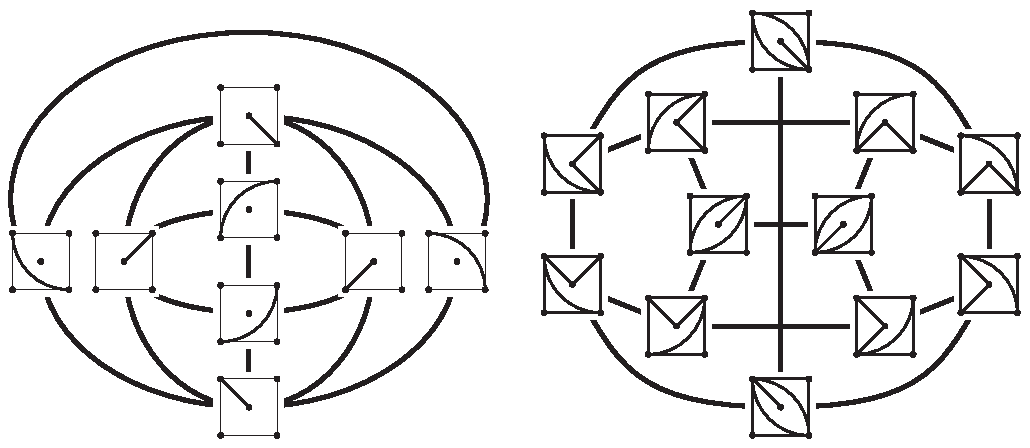
\includegraphics[scale=.95]{wigglyComplexSquare}}
\caption{The wiggly complex~$\wigglyComplex_P$ (left) and the wiggly flip graph~$\wigglyFlipGraph_P$ (right) of~$P$.}
\label{fig:wigglyComplexSquarre}
\end{figure}
\end{definition}

%Observe that it is not even clear from \cref{def:wigglyComplexPointSet} that the wiggly complex~$\wigglyComplex_P$ is a pure pseudomanifold (hence that the wiggly flip graph~$\wigglyFlipGraph_P$ is well-defined).
%However, we make the following ambitious conjecture.

\begin{conjecture}
\label{conj:polytopality}
For any point set~$P$ in the plane, the wiggly complex~$\wigglyComplex_P$ is the boundary complex of a simplicial polytope.
\end{conjecture}

\cref{conj:polytopality} holds in two extreme situations: the wiggly complex~$\wigglyComplex_P$ is realized
\begin{compactitem}
\item by the wigglyhedron of~\cref{thm:wigglyhedron} when the point set~$P$ is alogned, and
\item by the pseudotriangulation polytope of~\cite{RoteSantosStreinu-polytope}, realizing the flip graph on the original pseudotriangulations of~\cite{PocchiolaVegter,RoteSantosStreinu-pseudotriangulations}, when the point set~$P$ is in general position.
\end{compactitem}

\newpage
\section{Categorical representation theory}
\label{sec:representationTheory}


\newpage
%% if you use biblatex then this generates the bibliography
%% if you use some other method then remove this and do it your own way
\printbibliography



\end{document}
